\documentclass[tikz,border=10pt]{standalone}
\begin{document}
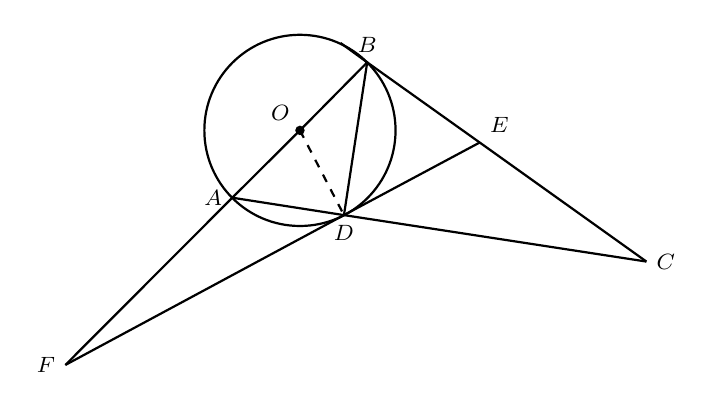
\begin{tikzpicture}[line width=0.8pt, line join=round, font=\fontsize{8}{9.6}\selectfont]
\coordinate (A) at (-1.571,0.117);
\coordinate (B) at (0.142,1.836);
\coordinate (C) at (3.688,-0.694);
\coordinate (D) at (-0.153,-0.104);
\coordinate (E) at (1.571,0.818);
\coordinate (F) at (-3.691,-2.007);
\coordinate (O) at (-0.712,0.972);
\coordinate (GeoTailB) at (-0.196,2.082);





\draw (O) circle[radius=1.214];


\draw (F)--(A)--(O)--(B)--(GeoTailB);


\draw (A)--(D)--(C);


\draw (B)--(E)--(C);


\draw (B)--(D);


\draw (F)--(D)--(E);


\draw[dashed] (O)--(D);


\fill (O) circle[radius=0.060];


\node[left] at (F) {$F$};
\node[above] at (B) {$B$};
\node[above left] at (O) {$O$};
\node[left] at (A) {$A$};
\node[below] at (D) {$D$};
\node[above right] at (E) {$E$};
\node[right] at (C) {$C$};
\end{tikzpicture}
\end{document}